% !TeX spellcheck = en_GB
\chapter{Implementation and Testing} % Realisierung und Test
\epigraph{Any fool can write code that a computer can understand. Good programmers write code that humans can understand.}{Martin Fowler}


\section{Development Setup}

Figure~\ref{fig:development-setup} illustrates the development setup in the form of an UML deployment diagram.
A developer connects via his browser to the reverse proxy that serves the XMPP-Grid Broker web application.
The HTTP connection from the client to the server is secured using mutual TLS authentication.
The same reverse proxy also routes the XMPP connections.
The client also authenticates to the proxy using mutual TLS authentication, and the proxy afterwards establishes a TLS connection to the XMPP server using his client certificates.
The reasons for this setup is described in more detail in Section \fullref{encountered-problems}.

\begin{figure}[h]
    \centering
    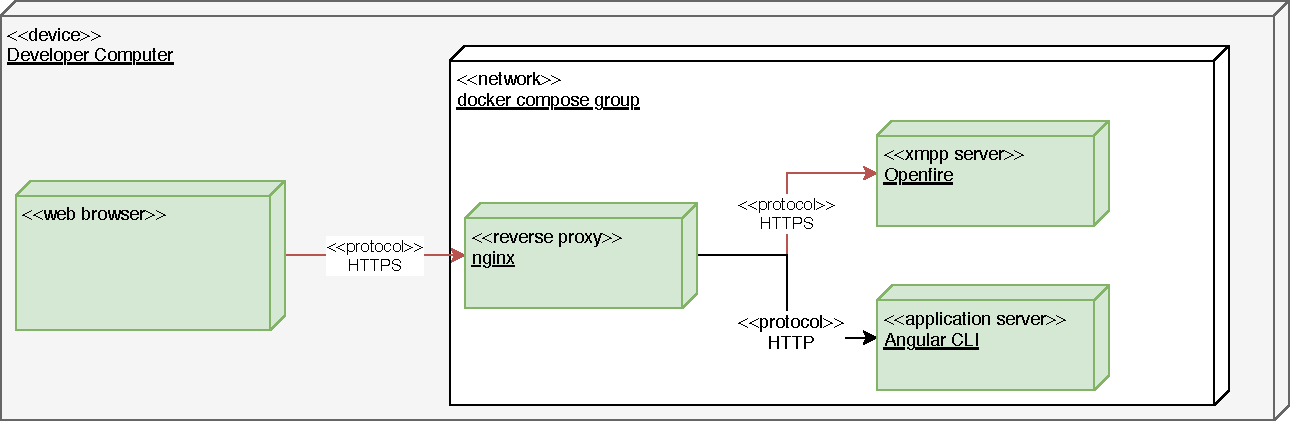
\includegraphics[width=1\linewidth]{resources/development-setup-uml}
    \caption{UML Deployment Diagram presenting the development setup}
    \label{fig:development-setup}
\end{figure}

As the previously described structure is not trivial, the guiding principle for our development setup was to maximise automation and minimise manual setup and configuration efforts. This principle is the basis for a durable software.
We decided on a docker and docker-compose\footnote{\url{https://www.docker.com/}} based stack that provides a correctly configured Openfire instance, a preconfigured nginx\footnote{\url{https://www.nginx.com/}} instance as well as client and server certificates.
Everyday tasks such as generating new certificates or building and testing the application and documentation were automated as bash scripts.

The efforts invested in this docker setup proved valuable when we began to write integration tests that run in the same environment.

We deliberately decided to run unit tests outside of the docker environment as unit tests are executed more often, and the additional docker-overhead would, therefore, be unnecessarily expensive.
Also, debugging is more straightforward without any indirections.

\section{Encountered Problems}\label{encountered-problems}

\subsection{Limitations of \emph{\fullref{sec:requirement-multiple-administrators}}}\label{sec:limitations-of-requirement-multiple-administrators}

Requirement \ref{sec:requirement-multiple-administrators} states that multiple administrators should be able to access the application.

When authenticating users with SASL EXTERNAL, the client certificate extension field `xmppAddr' is interpreted as user \gls{jid} by the \gls{xmpp} server.

In practice, most \gls{xmpp-grid} \gls{broker} deployments will require an HTTP proxy in front of the \gls{xmpp} server as security measure\footnote{
More information on this can be found in Section~\fullref{sec:implemented-web-application-topology}.}.
Usually, the HTTP proxy can also be used to serve the \gls{broker} application.
Such an HTTP proxy might also accept multiple different client certificates.

If the client connects to the \gls{xmpp} server over secure WebSockets (WSS) in combination with SASL EXTERNAL, the WebSocket URL must already be authenticated, as most browsers do not permit certificate selection on background requests\footnote{\url{https://bugs.chromium.org/p/chromium/issues/detail?id=329884\#c24}}.
This might be achieved by serving the \gls{broker} from the same domain or by using client certificate policies\footnote{\url{https://support.google.com/chrome/a/answer/6080885?hl=en\#manage-certs}}.

As the proxy intercepts the TLS connection, it must verify the client certificate sent by the browser and establish a connection to the \gls{xmpp} server using a client certificate as well.
Therefore, the `xmppAddr' field of the proxy's client ceritifcate is used by the \gls{xmpp} server.
If multiple users should be differentiated on the \gls{xmpp} server, an HTTP proxy might choose different client certificates for connecting to the \gls{xmpp} server based on the web browser's client certificate `xmppAddr'.


\subsection{Limitations of \emph{\fullref{sec:requirement-audit-trail}}}

Actions of administrators should be traceable with an audit trail according to requirement \ref{sec:requirement-audit-trail}.

As outlined in Section~\ref{sec:limitations-of-requirement-multiple-administrators}, practical deployments of \gls{xmpp-grid} \glspl{broker} will mostly use a HTTP proxy.
Additionally, to handling the client authentication, the proxy can be used to keep an audit trail of client requests.
These requests can then be correlated with the query log on the \gls{xmpp} server.

Creating audit trails on the client side does not provide additional safety, as users might prevent trail entries by manipulating the client application.
Therefore, no such mechanism was implemented.


% - Logout (TLS)
% - Initial Topic Consumers and Providers + Initial Topic Consumers and Providers => 2 Step Process!
% - Openfire:
%   - Lost updates with OpenFire
%   - falsche Felder - speziell pubsub#node_type
%   - vgl. https://discourse.igniterealtime.org/t/wrong-field-type-of-pubsub-node-type-and-how-to-update-it/81596
% -> Fehlende Methoden/Funktionalität im Standard
%   - "Liste alle Topics" -> Geht nur hierarchisch
%   - Filtering von Persisted Items

\section{Code Quality}
As our \gls{xmpp-grid} \gls{broker} implementation is intended to be a maintainable, production-ready application rather than a prototype, we placed much emphasis on code quality.
The measures taken can broadly be divided into three categories: technical measures, strategic decisions and processes.

\subsubsection{Technical Measures and Strategic Decisions}
Using Angular and the default Angular CLI was mostly a strategic decision.
Deviating as less as possible from the standard configuration ensures long-term maintainability and relatively straight-forward upgrades to newer Angular versions.
Another benefit of the Angular CLI project setup is that it comes with ``codelyzer''\footnote{\url{http://codelyzer.com/}} (including ``tslint'') for static code analysis and style linting.

Apart from the built-in linting mechanism, we followed Angular's Style Guide~\cite{angular-style-guide}.
Using the JetBrains IDEs (IntelliJ Ultimate and Webstorm)\footnote{\url{https://www.jetbrains.com/}} turned out to be particularly helpful as they give quick feedback for frequent mistakes and even violations of the Angular Style Guide.

We would have prefered to use more tools, especially for code metrics such as Lack of Cohesion of Methods (LCOM), and Afferent/Efferent Coupling.
However, we were not able to find such tools that were actively maintained and work with TypeScript.

\subsubsection{Processes}

On the process side, we tried to work test driven as much as possible.
Doing so turned out to be harder than expected as Angular's component testing infrastructure and the actual calls are sometimes wide apart (see Section~\fullref{sec:testing}).

Another process we heavily relied on were code reviews.
Each change, for the documentation and code, was reviewed using GitHub pull-requests\footnote{\url{https://www.github.com/}}.
In most cases, minor changes were detected and addressed during these reviews.
Continuous integration with TravisCI\footnote{\url{https://travis-ci.com/}} ensured that these changes never contained compilation errors or failing tests.

We also regularly discussed architectural and structural questions in our retrospectives and standup meetings.

In general, writing clean, modular and testable code has been our main priority.

\section{Testing}\label{sec:testing}

Good tests are inevitable for long-lived software projects.
They help developers to ensure that everything (still) works as expected after a change.
For the \gls{xmpp-grid} \gls{broker}, we focused on unit and end-to-end tests.
Following the principles of the test pyramid \cite{Cohn:2009:SAS:1667109}, we wrote many cheap and fast unit tests verifying the fundamental behaviour and fewer expensive and complex end to end tests.

\subsubsection{Unit Tests}

Testing the Angular Services was rather straightforward just by using jasmine and its mocking functionality.
We deliberately abstained from using Angulars testing framework for these services to keep them simple and comprehensible.
However, most of the services mainly send and receive XMPP-commands for which integration or end to end tests are required.

Writing tests for Angular Components, which require actual rendering a web browser, was not always essential.
To have fine-grained control and to be able to conduct tests, Angular provides a rather complex set of testing tools.
Because of this indirection, tests are conceptually not identical with the actual Angular application, making test driven development harder if not impossible.

\subsubsection{End to End Tests}

The end-to-end tests were written using Protractor, Angulars official end-to-end testing framework.
Protractor starts the development setup and verifies the application using a remote-controlled browser.

End-to-end tests are usually more challenging to write than unit tests, as different types of race conditions and varying delays to backend applications can occur.
Protractor usually resolves these issue due to its use of Zone.js, a library that creates ``execution context[s] that persists across async tasks'' called Zones.
To create Zones, Zone.js intercepts most web browser events, like HTTP requests.~\cite{zone-js-readme}

Because Zone.js is aware of all open HTTP requests, protractor can wait until a request and document change has completed before continuing with test execution.

However, due to our use of BOSH in the end-to-end tests\footnote{See Section~\fullref{sec:implemented-web-application-topology}}, we could not benefit from the Zone.js change detection.
BOSH uses HTTP long polling to communicate with the XMPP server, which leads to a Zone that always has open requests~\cite{xep-0124}.

Therefore, we had to manually implement waiting conditions, which proved to be difficult due to unstable web browser behaviour.

In our case, writing tests paid off quickly as they promptly caught many potential bugs introduced by small changes and refactorings.

\section{Documentation}
% - Installation
% - Benutzerdokumentation
% - Zielerreichung
% - Architectural Decisions